\section{Numerical Experiments}\label{sec:crqi:experiments}
In this section we discuss different numerical examples to better
understand the behaviour of CRQI. Throughout the section we will
always compare the method to classic RQI. All experiments were
executed in Matlab 9\todo{Cite matlab}. The criterion for convergence
was
$\norm*{\vec{r}^{(k)}} = \norm*{\mat{A}\vec{x}^{(k)} - \mu^{(k)}
  \vec{x}^{(k)}} < 10^{-8}$. The source codes for both classic and
complex RQI can be found in the Appendix. The methods are defined
slightly differently from the Algorithms given above. They both allow
to explicitly set the initial shifts $\mu^{(0)}$ and $\gamma^{(0)}$ to
specific values whereas in Algorithm~\ref{alg:rqi} and
Algorithm~\ref{alg:crqi:proj} the initial shifts are always
initialised as the Rayleigh Quotient of the initial vector and the
initial residual, respectively. In most of the examples below the
matrix $\mat{A}$ was a randomly generated sparse symmetric
$200 \times 200$ matrix. To simulate that a good approximation of the
initial vector is available we computed the full set of eigenvectors
collected as columns of the matrix $\mat{V}$. Next, a weight vector
$\vec{w}$ of uniformly distributed numbers between $0$ and $1$ is
created. One of the components is set to a higher value than the
others, \eg $w_{50} = 10$ (in most examples the index of the component
was also chosen randomly). The initial vector is then set to a
weighted linear combination of the eigenvectors, \ie
$\vec{x}^{(0)} = \beta \mat{V} \vec{w}$, where $\beta$ has to be
chosen such that $\vec{x}^{(0)}$ is normalised. Now, $\vec{x}^{(0)}$
is a vector with a strong component in the direction of the target
eigenvector and random (smaller) contributions in the directions of
the other eigenvectors.

The first example demonstrates the influence of the imaginary shift
$\gamma^{(k)} i$ on the convergence speed. We started by running two
versions of CRQI. The first uses
$\gamma^{(k)} = \norm*{\vec{r}^{(k)}}$, the second uses the square of
the residual norm. A plot of the residuals against the iteration
number of both these approaches together with the results using
classic RQI\footnote{Classic RQI is merely included for speed
  comparison. Since the eigenvalues of the test problem are closely
  spaced, in almost all of the examples classic RQI failed to converge
  to the right eigenvalue.} and a third approach described shortly is
given in Figure~\ref{fig:residuals}.

\begin{figure}[htpb]
  \centering
  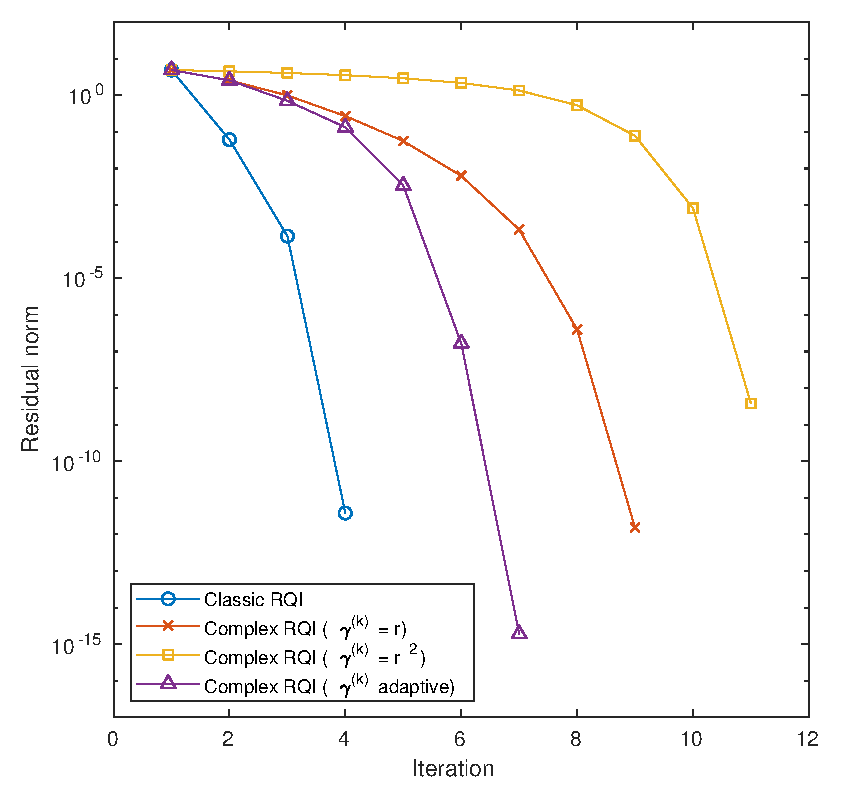
\includegraphics[width=0.7\textwidth]{Figures/crqi_residuals}
  \caption[Residuals for different choices of $\gamma^{(k)}$.]{Plot of
    residuals of Classic RQI, Complex RQI with
    $\gamma^{(k)} = \norm*{\vec{r}^{(k)}}$, Complex RQI with
    $\gamma^{(k)} = \norm*{\vec{r}^{(k)}}^2$ and Complex RQI with the
    imaginary shift chosen adaptively (see text). The last variantt
    seems to combine the adavantages of the second and third
    alternatives.}%
  \label{fig:residuals}
\end{figure}

We observe that in the initial phase of the iteration, the second
variant seems to be slower than the first. Altough it is not clearly
observable in the figure below, other examples suggested that during
the final steps of the iterations the second version was faster than
the first. Consequently, by combining both approaches and thus
changing the shift adaptively we expect faster convergence. The
results are also plotted in Figure~\ref{fig:residuals} and are in
accordance with the expectation. In this particular case, the shift
was changed adaptively according to
\begin{equation*}
  \gamma =
  \begin{cases}
    \norm*{\vec{r}} & \text{ if } \norm*{\vec{r}} \ge 1\,, \\
    \norm*{\vec{r}}^2 & \text{ if } \norm*{\vec{r}} < 1\,,
  \end{cases}
\end{equation*}
where we dropped the superscripts from $\gamma = \gamma^{(k)}$ and
$\vec{r} = \vec{r}^{(k)}$. In the following, when we speak of CRQI we
mean CRQI performed with this adaptive choice of imaginary shifts.

Running the same experiment but increasing the component of the
initial vector in the direction of the target eigenvector it showed
that the number of additional steps required by CRQI diminshed. For
eigenvectors that were very close to the target sometimes both classic
RQI and complex RQI finished within the same number of iterations and
while CRQI generally produced the correct eigenpair, classic RQI
usually failed to do so.

\begin{figure}[htpb]
  \centering
  \begin{subfigure}[b]{0.475\textwidth}%
    \centering
    \includegraphics[width=\textwidth]{Figures/crqi_varyingshift__initvec_small_direction_70deg_negative}%
    \caption{{\small Small component in target direction, negative
        eigenvalue}}%
    \label{fig:varying shift small negative}
  \end{subfigure}%
  \hfill
  \begin{subfigure}[b]{0.475\textwidth}%
    \centering
    \includegraphics[width=\textwidth]{Figures/crqi_varyingshift__initvec_small_direction_70deg}%
    \caption{{\small Small component in target direction, positive
        eigenvalue}}%
    \label{fig:varying shift small positive}
  \end{subfigure}
  \vskip\baselineskip
  \begin{subfigure}[t]{0.475\textwidth}%
    \centering
    \includegraphics[width=\textwidth]{Figures/crqi_varyingshift__initvec_suffctl_big}%
    \caption{{\small Sufficiently big component in target direction}}%
    \label{fig:varying shift big}
  \end{subfigure}
  \hfill
  \begin{subfigure}[t]{0.475\textwidth}%
    \centering
    \includegraphics[width=\textwidth]{Figures/crqi_varyingshift__initvec_random}%
    \caption{{\small Random initial vector}}%
    \label{fig:varying shift random}
  \end{subfigure}
  \caption[RQI and CRQI wiith varying initial shifts]{Plot of initial
    real shift against the computed eigenvalue using classic RQI and
    CRQI. The dotted area encloses the initial shifts that lie in the
    spectrum of $\mat{A}$. In the first two examples the initial
    vector had only a small component in the direction of the target
    eigenvector. }
  \label{fig:vary shift}
\end{figure}

Further investigation revealed that the behaviour as in
Figure~\ref{fig:varying shift small positive} and
Figure~\ref{fig:varying shift small negative}
%%% Local Variables: 
%%% mode: latex
%%% TeX-master: "../../main"
%%% End:
